\documentclass[11pt,a4paper]{article}
\usepackage[utf8]{inputenc}
\usepackage[portuguese]{babel}
\usepackage[T1]{fontenc}
\usepackage[ddmmyyyy]{datetime}
\usepackage[margin=2cm]{geometry}
\usepackage{amsfonts}
\usepackage{amsmath}
\usepackage{amssymb}
\usepackage{amsthm}
\usepackage{biblatex}
\usepackage{csquotes}
\usepackage{graphicx}
\usepackage{mathtools}
\usepackage{thmtools}
\usepackage{titling}
\usepackage{xcolor}
\usepackage[unicode]{hyperref}

\pdfsuppressptexinfo=7

\graphicspath{{e-folio/e-folio-a/imagem}}
\addbibresource{bibliografia.bib}

% Ambientes de provas e demonstrações
\newtheorem{theorem}{Teorema}[section]
\newtheorem{proposition}{Proposição}[theorem]
\renewcommand\qedsymbol{\textbf{q.e.d.}}

% Dados
\author{Carlos Augusto Gonçalves Collaço e Pinto Machado}
\newcommand{\numeroEstudante}{2200909}
\newcommand{\UC}{Elementos de Análise Infinitesimal I}
\newcommand{\codigoUC}{21030}
\newcommand{\docentes}{Maria João Oliveira}
\newcommand{\curso}{Licenciatura em Matemática e Aplicações}
\newcommand{\turma}{2}
\newcommand{\anoLectivo}{2023-2024}
\date{\today}

\pagenumbering{arabic}

\hypersetup{
	pdfsubject={\UC},
	pdftitle={E-fólio A - \numeroEstudante},
	pdfauthor={Carlos Pinto Machado},
	pdfproducer={},
	pdfcreator={}
}

\makeindex

\newcommand{\exercicio}{
	\addtocounter{section}{1}
	\setcounter{subsection}{0}
	\section*{\arabic{section}}
	\addcontentsline{toc}{section}{Exercício \arabic{section}}
}


\begin{document}

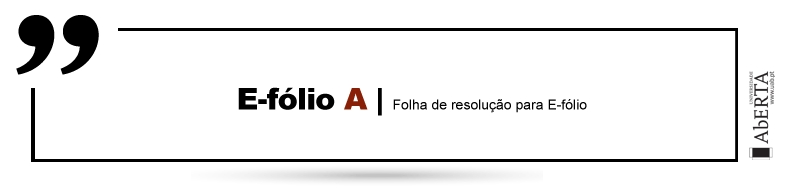
\includegraphics[width=\textwidth]{e-folio-a.jpg}

\paragraph{\textbf{UNIDADE CURRICULAR:}} \UC

\paragraph{\textbf{CÓDIGO:}} \codigoUC

\paragraph{\textbf{DOCENTE:}} \docentes

\paragraph{\textbf{NOME:}} \theauthor

\paragraph{\textbf{N.º DE ESTUDANTE:}} \numeroEstudante

\paragraph{\textbf{CURSO:}} \curso

\paragraph{\textbf{DATA DE ENTREGA:}} \thedate


\clearpage


\clearpage

\nocite{*}
\printbibliography[heading=bibintoc,title={Bibliografia}]

\end{document}
